\documentclass[12pt,letterpaper]{article}

%%%%% CAMBIAR LA PRIMERA LINEA POR LA SIGUIENTE PARA LA MEMORIA DE PROYECTO %%%%%
%\documentclass[12pt,letterpaper,oneside]{book}

% Paquetes basicos ...
\usepackage[utf8]{inputenc} % OJO!!!  => MANTENER ESTA LINEA PARA FACIL CONVERSION A WORD EN EL FUTURO ...
\usepackage[spanish]{babel}
\usepackage{graphicx} 
\usepackage{array}
\usepackage{tabularx}
\usepackage{amssymb, amsmath}

% Paquetes extras ... 
\usepackage{subfigure}
\usepackage{color}
\usepackage{anysize} 
\usepackage{breakcites}
\usepackage{enumitem}


\begin{document}
\marginsize{2.5cm}{2cm}{2cm}{2cm} 

% Para que no aparezca la numeracion en el pie de pagina de todo el documento ...
%\pagestyle{empty}


%%%%%% ******  INICIO CARATULA ***** %%%%%%%%%
% Especificaciones de la caratula PPG
\begin{titlepage}
\begin{center}
\vspace*{-0.5in}
\begin{large}
\textbf{UNIVERSIDAD MAYOR DE SAN ANDRÉS}\\
\vspace*{0.15in}
\textbf{FACULTAD DE INGENIERÍA}\\
\vspace*{0.15in}
\textbf{CARRERA DE INGENIERÍA ELECTRÓNICA}\\
\vspace*{0.1in}
\end{large}
% Logo UMSA
\begin{figure}[htb]
\begin{center}

\includegraphics[width=8cm]{umsa.jpg}
\end{center}
\end{figure}
\begin{Large}
\textbf{PERFIL DE PROYECTO DE GRADO} 
\end{Large}
\vspace*{0.4in}

\begin{normalsize}
\textbf{`` Detección de carril usando redes neuronales convolucionales y aprendizaje profundo''} \\
\end{normalsize}



\vspace*{0.2in}


\begin{large}
\textbf{POSTULANTE:} JOSE EDUARDO LARUTA ESPEJO\\
\end{large}

\begin{large}
\hspace{0.08in} \textbf{TUTOR:} JAVIER SANABRIA GARCIA\\
\end{large}

\begin{large}
\hspace{0.44in} \textbf{D.A.M.:} ALFONSO JURADO VISCARRA\\
\end{large}

\vspace*{0.2in}



\begin{normalsize}
LA PAZ, AGOSTO 2018\\
\end{normalsize}
\end{center}
\end{titlepage}


\thispagestyle{empty}
% Generacion del indice
\tableofcontents
\newpage

%%%%%% ******  FIN CARATULA ***** %%%%%%%%%

% Contenido del PPG
% NOTA: presionar F11 para que se actualicen las citas bibliograficas ...

\section{Introducción}

Los vehículos autónomos han pasadoe de ser un tema de ciencia ficción a convertirse una realidad cada vez más 
cercana. Si bien existe un recorrido muy largo para llegar a implementar sistemas completamente autónomos en las calles, 
lose recientes avances en la tecnología junto con el interés económico de grandes empresas y corporaciones en el mundo 
ha hecho posible incluir diversos niveles de autonomía a vehículos con fines de uso doméstico e industrial con éxito.

Una de las áreas que más se ha nutrido de los recientes avances es el área de la visión artificial o visión por computador; 
resolviendo con facilidad tareas de una complejidad muy alta, como la detección y reconocimiento de objetos. 
Este crecimiento, en gran parte, se ha debido al desarrollo y optimización de las redes neuronales, las cuales se han 
constituido en una herramienta con muchas potencialidades y aplicaciones por la forma en la que se procesa la información 
y su capacidad para generalizar tareas complejas en base a una gran cantidad de datos de entrenamiento. En específico, 
las redes neuronales convolucionales han podido revivir al campo de la visión artificial gracias a la forma eficiente 
en la que procesa imágenes o matricies multidimensionales y la capacidad de crear representaciones internas a partir de imágenes.

La visión artificial juega un papel muy importante en el desarrollo de vehículos autónomos por cuanto permite 
procesar imágenes digitales provenientes de cámaras instaladas en los mismos vehículos y extraer información 
valiosa para la navegación y la conducción, como ser la detección de carril, peatones, signos de tránsito, otros vehículos, 
etc. Esta utilidad hace posible diversas oportunidades de investigación y desarrollo de algoritmos y sistemas de visión 
artificial orientados a conducción autónoma.

El presente proyecto se centra en el desarrollo de un sistema de detección de carril basado en visión artificial para 
la generación de comandos de control para la conducción autónoma de un vehículo doméstico con un modelo de locomoción 
de Ackerman. Se intenta desarrollar un sistema “fin a fin” que consta de un modelo que genera comandos de control a 
partir de un estímulo visual solamente.

\section{Antecedentes}

En Bolivia existe más de un millón de automotores y la gran mayoría son de uso privado. El parque automotor va 
en crecimiento y junto con él temas de impacto ambiental que van en desmedro de la calidad de vida de la población 
como por ejemplo: polución del aire, contaminación sonora o mal uso de espacios públicos. En este entendido, el 
desarrollo de vehículos autónomos surge como una oportunidad para solucionar algunos de estos problemas y mejorar 
la calidad de vida de la población.

El primer intento de desarrollo de un sistema de conducción autónomo “fin a fin” fue llevado a cabo por la Agencia 
de Proyectos de Investigación Avanzada en Defensa (DARPA) con un proyecto conocido como el Vehículo Autónomo DARPA o 
DAVE en el cual un vehículo radio controlado a escala tenía la tarea de conducir a través de un entorno escabroso. 
El vehículo DAVE fue entrenado a partir de horas de conducción humana en entornos similares pero no idénticos. Los datos 
de entrenamiento incluyeron imágenes de dos cámaras de video y comandos de control generados por un operador humano. 

Luego de esto, el primer hito en el desarrollo de un sistema completamente autónomo vino con la organización del DARPA 
“Grand Challenge” en el cual equipos de varias universidades, institutos de investigación y empresas tuvieron que 
enfrentar el difícil reto de desarrollar un sistema capaz de controlar un vehículo doméstico para que se maneje solo a 
través de una carretera ripiada en medio del desierto de Arizona. Dentro las 2 versiones del Darpa Grand Challenge 
destacaron los proyectos de universidades como Stanford con el robot Stanley que fue el primer vehículo en recorrer 
mas de 170 kilómetros en una carretera ripiada de manera completamente autónoma. 

El éxito de los proyectos que participaron en el grand challenge sentó un gran precedente en el desarrollo de lo que 
ahora se conoce como Self Driving Car. De hecho, muchos de los equipos participantes de este concurso se constituyen 
ahora como existosas empresas de desarrollo o coadyuvan en iniciativas privadas de gigantes de la tecnología 
como Google, Uber o Nissan.

La regulación define varios niveles de autonomía en vehículos terrestres, aéreos y acuáticos yendo desde un control 
completamente manual, normalmente observado en vehículos completamente mecánicos, pasando por asistencias al control 
hasta llegar a un vehículo completamente autónomo en todas sus tareas

En la actualidad, existen varias iniciativas en el desarrollo de los self Driving Cars, siendo una de las más 
importantes la empresa Waymo, dependiente de Google a través de su empresa Pública Alphabet. Waymo, ha aprovechado 
el uso de tecnologías emergentes de sensado como el LIDAR para mejorar el mapeo y la navegación a través de algoritmos 
de fusión de sensores.

Una de las tareas más importantes dentro de un self driving car es la detección y mantención del carril del 
vehículo. Fabricantes de vehículos automotores han incluido con éxito sistemas de asistencia al conductor para la 
mantención del carril usando cámaras digitales y visión artificial para poder detectar la posición del automóvil con 
respecto al carril. Estos sistemas se consideran fundamentales en sistemas de conducción autónoma.

Entre las técnicas empleadas para lograr la tarea de detección y mantención del carril en una avenida o carretera 
se pueden encontrar diversos enfoques entre los cuales podemos destacar los siguientes 2:

\begin{itemize}
    \item Fusión de sensores e ingeniería de ``características''
    \item Aprendizaje ``Fin a Fin''
\end{itemize}
%*******************JUSTIFICACION*******************

\section{Justificación del Proyecto}

\subsection{Justificación técnica}
El proyecto se justifica desde el punto de vista técnico a partir de las técnicas y procedimientos explorados 
en el mismo para implementar un sistema de visión y control asistido basado en una red neuronal convolucional. 
Usualmente, el análisis de la aplicabilidad de una red neuronal involucra solamente la prueba sobre un dataset 
genérico donde se evalúa su rendimiento analizando el error de clasificación y pérdidas. En este caso, se plantea el 
flujo de trabajo completo orientado a la implementación en un prototipo a escala usando técnicas convencionales en 
el análisis y diseño de sistemas de visión artificial así como también la implementación del mencionado sistema en 
una plataforma de cómputo embebida.

Las tecnologías a ser usadas deberán tener la característica de pertenecer a los estándares actuales en la 
investigación e industria, esto con el fin de ser replicable y extensible en futuros proyectos.

\subsection{Justificación académica}

Desde el punto de vista académico, el proyecto se justifica en el entendido del uso de técnicas y procedimientos 
de ingeniería para el análisis y diseño de un sistema de aprendizaje “fin a fin” usando redes neuronales. Tales 
técnicas y procedimientos incluyen la definición de la arquitectura de la red neuronal, el entrenamiento y el análisis 
del rendimiento de la misma. Así como también el dimensionamiento de los componentes de cómputo embebido para el 
prototipo y la implementación de los sistemas de control de bajo nivel para el mismo. Tales técnicas y 
procedimientos se corresponden de manera integral con los conocimientos adquiridos a lo largo de la carrera 
de Ingeniería Electrónica en sus distintas asignaturas.


%******************ANALISIS DE LA PROBLEMATICA*********************
%------ TODO: completar esta parte ------------- %
\section{Análisis de la problemática y \\
planteamiento del problema}
\subsection{Análisis de la problemática}
% PROBLEMATICA: Conjunto de aspectos que causan problemas en un PG.
% ANALISIS DE LA PROBLEMATICA: Determinacion de las causas sus efectos y sus relaciones, vinculados con los aspectos problematicos de la idea del proyecto.  
% ****Es el analisis de las cuestiones discutibles que requieren de una solucion en el PG.

Se han estudiado diferentes enfoques para lograr solucionar la tarea de 
conducción autónoma para vehículos domésticos. Normalmente, la salida del 
sistema se expresa como una serie de comandos de control de aceleración y dirección 
del volante del vehículo. Estos comandos se pueden obtener de diversas maneras dependiendo 
el nivel de robustez y abstracción que el sistema requiere. Muchos sistemas 
se basan en la fusión de distintos tipos de sensores y fuentes de información como ser 
mapas satelitales, GPS, sensores láser y cámaras. La combinación de esta información 
es procesada y fusionada mediante distintos algoritmos de filtrado tales como el filtro de kalman. 
La característica de este tipo de sistema es que se puede expresar como una serie de etapas 
de procesamiento mediante el cual la información fluye y se transforma, cada una de las etapas es 
diseñada e implementada en base a conocimiento específico y con requerimientos y limitaciones específicas 
de la tarea que realiza. 

Si bien el enfoque anteriormente mencionado ha logrado conseguir importantes avances y resultados 
muy prometedores, involucra un gran esfuerzo a la hora de diseñar cada una de las etapas independientemente 
para luego hacer que funcionen todas juntas y cumplan la tarea asignada. Este proceso usualmente requiere 
de un equipo de expertos que sea capaz de realizar las tareas de diseño de las etapas o módulos del sistema 
y el de la integración de los módulos en un solo sistema funcional. Este enfoque, pese a que ha demostrado ser 
una forma efectiva de trabajo para diversos problemas, tiene la desventaja de requerir muchos 
recursos y tiempo para poder lograr un sistema funcional. 


%Descripcion de la labor de Desminado Humanitario

\subsection{Planteamiento del problema}
% PLANTEAMIENTO DEL PROBLEMA: Tiene que ver con enfocar la solucion de los aspectos problematicos tratados, 
% desde su situacion inicial hasta su situacion final deseada.

Considerando a la tarea de conducción autónoma como un sistema de procesamiento de datos, se debe tener en 
cuenta varios aspectos concernientes tanto al diseño como a la implementación de dichos tipos de sistemas. Una 
de las principales características es que tradicionalmente el flujo de la información pasa por varias etapas.

En el área de visión por computadora para tareas de conducción autónoma, normalmente se sigue el siguiente flujo:

\begin{enumerate}
    \item \textbf{Extracción de características.} Esta etapa incluye el preprocesamiento y transformación de la imagen 
    en un conjunto de características de distinta índole. Estas características se suelen llamar también descriptores 
    y sirven para describir los aspectos más relevantes de la imagen para la tarea final, por ejemplo, la detección de bordes. 
    La extracción de características también se usa para reducir la dimensionalidad inicial de la imagen a una más tratable y 
    amigable con el poder de procesamiento disponible. Las características o descriptores a usarse se definen manualmente por 
    medio de conocimiento experto y se afinan de la misma manera.

    \item \textbf{Algoritmo predictor.} Esta etapa incluye típicamente un algoritmo de aprendizaje previamente entrenado con un conjunto 
    de datos adecuado, permite realizar distintas tareas de alto nivel sobre los descriptores obtenidos de la imagen. Estas 
    descripciones de alto nivel incluyen normalmente tareas de detección, clasificación o regresión.

    \item \textbf{Adecuación de los datos de salida.} La información extraída de la anterior etapa debe procesarse para poder ser traducida 
    a comandos de control que actuen directamente con las etapas de bajo nivel del vehículo, es decir la etapa de actuación y potencia.
\end{enumerate}


  - complejidad
  - lentitud en la implementacion
  - 
%------------------
\section{Objetivos}
\subsection{Objetivo General}

Diseñar un sistema de aprendizaje “fin a fin” para la generación de comandos de 
dirección en la tarea de conducción autónoma de vehículos domésticos basado en 
visión artificial y redes neuronales convolucionales.

\subsection{Objetivos Específicos}
Para alcanzar el objetivo general será necesario:

\begin{itemize}
    \item Investigar y evaluar requerimientos específicos para el sistema.
    \item Diseñar una plataforma de prueba en hardware con características similares a las de un vehículo doméstico real.
    \item Diseñar la arquitectura de una red neuronal capaz de cumplir con la tarea de generación de comandos 
    de control para un vehículo autónomo.
    \item Realizar pruebas de rendimiento y análisis comparativos en base al sistema implementado.
    \item Proponer un prototipo funcional en el que se pueda apreciar los alcances del sistema.
\end{itemize}


\section{Alcance}

Dentro de los alcances del proyecto se puedencitar los siguientes
aspectos:

\begin{itemize}
    \item Recopilación de información de distintas fuentes en 
    en trabajos de investigación.
    \item El desarrollo de un prototipo funcional a escala con 
    locomoción de Ackerman.
    \item El diseño electrónico del circuito de control y comunicación de
    la Computadora de Abordo.
    \item Investigación de arquitecturas y plataformas de software para el
    diseño y despliegue de robots móviles y tareas de conducción autónoma.
    \item El diseño de la arquitectura de la red neuronal en base a 
    especificaciones de funcionamiento, desempeño y plataforma de hardware.
    \item Uso de algoritmos de preprocesamiento de datos y funciones
    de agregación de datos previos al entrenamiento de la red neuronal.
    \item El entrenamiento de la red neuronal en un entorno externo a la OBC.
    \item El análisis de los errores de entrenamiento y validación de la red neuronal.

\end{itemize}

\section{Límites}
El sistema, por su parte, contará con ciertas restricciones detalladas a 
continuación:
\begin{itemize}
    \item En la recopilación de información y fuentes se 
    considerará principalmente investigaciones y trabajos relacionados
    con tareas de aprendizaje "fin a fin" y redes neuronales convolucionales.
    \item El prototipo a escala servirá solamente para un análisis superficial 
    de la dinámica de un vehículo automotor doméstico tomando como punto 
    de inicio modelos matemáticos simplificados y limitaciones de rangos de trabajo dentro 
    de dichos modelos.
    \item la electrónica de los sistemas de control y percepción estará 
    diseñada específicamente para el modelo a escala y las limitaciones anteriormente
    mencionadas.
    \item Se explorarán exclusivamente plataformas, librerías y herramientas
    de cógo abierto y con licencias de uso no privativas.
    \item El diseño de la arquitectura de la red neuronal estará orientado a 
    tareas de aprendizaje supervisado y aproximación de funciones.
    \item tanto la arquitectura de la red como los hiperparámetros de 
    la misma estarán acotados considerando las limitaciones de memoria y capacidad 
    de procesamiento ofrecidos por la plataforma de cómputo o Computadora
    de Abordo disponible.
    \item La recolección de datos estará enfocada y definida por el prototipo
    a implementar.
\end{itemize}
\section{Solución Propuesta}

La solución propuesta se compone de un sistema capaz 
Una propuesta inicial del diseño de un esquema de control por módulos para un sistema multi-robot destinado 
a labores de Desminado Humanitario se describe en las Figuras \ref{fig:esquema1} y \ref{fig:esquema2}, no obstante 
la misma podría ser sujeta de modificaciones en función de aspectos relevantes que puedan surgir 
en el desarrollo del trabajo...

%%%% Figura 1 %%%%%%
\begin{figure}[h!] 
\centering
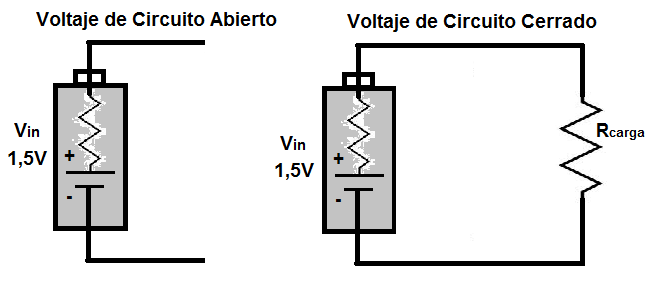
\includegraphics[width=0.5\textwidth]{esquema1}
\caption{La leyenda viene aca ...}
\label{fig:esquema1}
\end{figure}


%%%% Figura 2 %%%%%%
\begin{figure}[h!] 
\centering
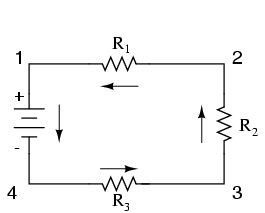
\includegraphics[width=0.5\textwidth]{esquema2}
\caption{La leyenda viene aca ...}
\label{fig:esquema2}
\end{figure}







 
 





\section{Temario del Proyecto}
A continuación se presenta el temario tentativo de la memoria del proyecto, considerando los posibles contenidos, sin un detalle exhaustivo de los mismos puesto que podría ser una limitante en la estructura final. Inicialmente se considera la siguiente estructura:\\

\begin{itemize}

\item \textbf{Título.}

\item \textbf{Resumen.}

\item \textbf{Dedicatoria.}

\item \textbf{Agradecimientos.}

\item \textbf{Lista de Figuras.}

\item \textbf{Capitulo 1: Introducción}  

\item \textbf{Capitulo 2: Fundamentos del proyecto}  

\item \textbf{Capitulo 3: Marco práctico del proyecto} 

\item \textbf{Capitulo 4: Análisis y discusión de resultados}

\item \textbf{Capitulo 5: Conclusiones y recomendaciones}
\item \textbf{Referencias y bibliografía}

\item \textbf{Glosario de términos}

\item \textbf{Anexos}
%\renewcommand{\theenumi}{\thesection.\arabic{enumi}}
\end{itemize}

 
\section{Cronograma del Proyecto}

Diagrama Gantt ...




\section{Bibliografia}





\bibliographystyle{apalike}
\bibliography{referencias}
\end{document}
